%!TEX root = ../Touch Based Idris.tex
\section{Analysis of Visual and Touch Based Solutions}
\label{sec:Analysis}
\todo{insert screenshots of more or less all the solutions}
In this section, we evaluate a range of visual and touch based programming interfaces and languages. It is the goal of this phase
to... \todo{fill out. Something like: find out if the Idris editor should be
visual/textual, structured/free text, to what extend it should rely on touch
gestures}.

\subsection{Investigation Scope}
The amount of touch-based and visual programming languages and editors that have already been developed is quite large as can be seen from Eric Hosick's list.\,\cite{hosick2014} For this very reason it was important for us to define which types of existing solutions that are of interest.

As we are designing a high-level syntax for the programming language Idris, we
can define our target group to users that are familiar with dependently typed
languages. Plenty of experiments with visual languages for educational purposes
have been conducted (see Scratch section) \todo{ref (Pane et al., A. Myers,
Green)}, so we should only take more experienced programmers into consideration
when designing the user experience.

As Idris is general purpose we will not be investigating domain specific languages orplatforms unless elements of their syntax or IDE has potential of working with general purpose languages.

There are many visual workflow editors that basically use a collection of boxes and arrows to visualize state and actions. Author and Author \todo{insert ref} argue that purely visual languages like these do not scale well. Our focus has thus moved away from purely visual workflow languages to languages that only partially rely on visual syntax.
\todo{is this true?}

Still, with these limiting factors there are too many candidate solutions for us to analyze and evaluate them all. The following analysis consists of a selection of the existing solutions that we found most relevant to our study and mainly applies the heuristic evaluation technique by Nielsen\,\cite{nielsen1990heuristic}. Such an evaluation can give an idea of possible usability issues but I will not help discover them all. This suits our purpose, as it is our mission to get an overview of the major pitfalls as well as what generally works well when designing our solution. Furthermore, we are pursuing an entirely new type of touch-based, visual, and structured interface instead of bettering an existing one so analyzing a few existing solutions in depth does not make as much sense
as investigating a wide range more generally.

The thoroughness of our analyses also depend on something as practical as whether we have been able to install the tool/language on our machines. Some of the solutions in question are old or experimental only. In some cases the only thing available are conceptual descriptions by the
creators.\todo{maybe give DRAKON as example, which was really cool but only
available in Russian}

\subsection{Visual Programming Languages}
We will be investigating two Visual Programming Language (VPL) as well as Epigrams hybrid approach in this section.

\todo{We should have an explanation of Physics of Notation here. We just
reference it randomly in the text}

\subsubsection{Labview}
\label{subsub:Labview}
Labview is a development environment featuring the VPL, G, which is designed for dataflow programming and uses the popular ``boxes and wires'' abstraction, with boxes performing various functions, and wires leading data between the boxes. Labview also lets users combine simple widgets to build GUI programs, using the G language for logic. It is widely used in the scientific community, especially to work with data collected from sensors.
Figure \ref{fig:LabViewGettingStarted} shows a simple example of calculating a
triangle's area.

\begin{figure}
	\centering
		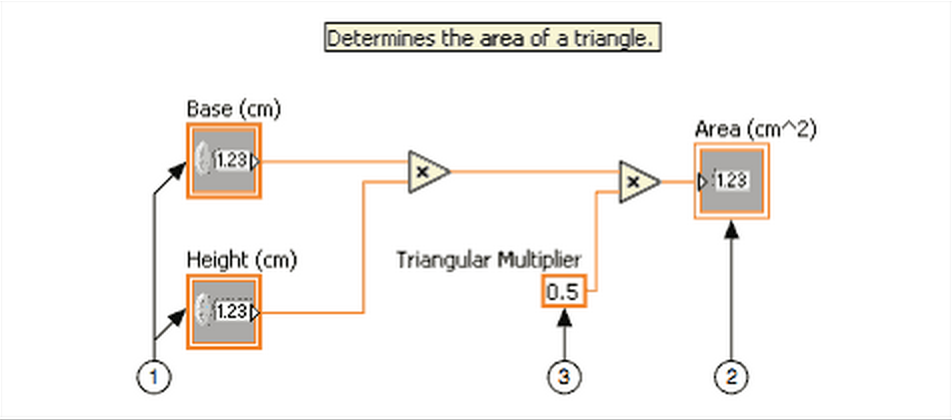
\includegraphics[width=110mm]{diagrams/LabView_screenshot.png}
	\caption{A simple LabView program from the tutorial\,\cite{LabView:GettingStarted}}
\label{fig:LabViewGettingStarted}
\end{figure}

Labview is often referenced in the literature of VPLs \todo{insert a couple of references}, so even though it is domain specific we find it interesting as a starting point for our investigation.

While complex programs in G can be initially overwhelming to even experienced programmers, Whitley and Blackwell \todo{WHITLEY AND ALAN F. BLACKWELL (ref)} show that seasoned Labview programmers prefer the visual syntax to a textual one.

It is interesting how Green and Petre \todo{(ref)} give Labview an overall positive response when evaluating it through the cognitive dimensions framework, it would almost certainly be viewed more negatively using the Physics of Notation framework\todo{ref}. Like UML, G does not make use of many of the principles, such as Visual Expressiveness, Perceptual Discriminability and Complexity Management.

\paragraph{Takeaways}
\begin{enumerate}
	\item One interpretation of Whitley and Blackwell's findings \todo{WHITLEY AND ALAN F. BLACKWELL (ref)} is that although Labview can be hard for programmers not used to the visual syntax, the higher learning curve pays off in the long run.
	\item The fact that Labview does not make use of the various principles of physical notation might help explain why newcomers find it daunting.
	\item The ``boxes and wires'' approach is good at indicating structure and could maybe be transfered to a more general purpose language representation such as IdrisTouch.
\end{enumerate}


\subsubsection{Scratch}
\label{subsub:Scratch}
Scratch is a visual programming language designed to be easy for beginners to use, facilitating the development of simple audio/visual programs. It is implemented as a web app, and features built-in tutorials, tips and help.
The language is built around a scene containing sprites. A scene can have multiple sprites, and each sprite can be governed by multiple scripts written in the Scratch visual language. The language itself consists of blocks of different shapes, colors and sizes. Scratch does not use the dataflow paradigm, as Labview does. Instead, one programs by snapping blocks together. As can be seen from Figure \ref{fig:ScratchProgram}, the blocks have different shapes, and only complementing shapes can be put together. Color is used to describe different types of blocks.

\begin{figure}
	\centering
		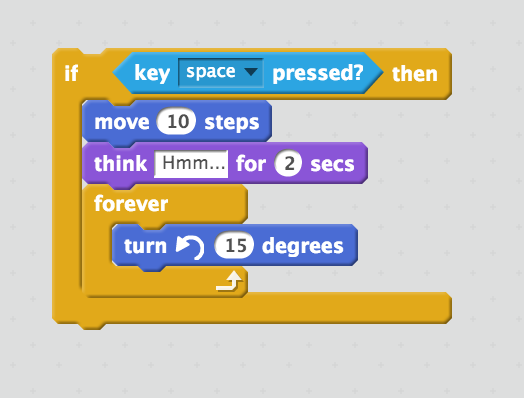
\includegraphics[width=60mm]{diagrams/ScratchProgram.png}
	\caption{A simple Scratch program that moves and spins the sprite if the space
	button is pressed.}
\label{fig:ScratchProgram}
\end{figure}

The user interface itself is a bit cluttered, and it is not immediately clear how the three main areas (scene, sprites, and scripts) interact. Once this has been discovered, however, it is reasonably easy to use. 
\todo{This paragraph needs to be more academic}

A wide range of solutions based on or similar to Scratch have been made over the years\,\cite{hosick2014}, but one is, in particular, interesting to us as it is a port of Scratch to the Apple iPad. It is called Hopscotch\,\cite{hopscotch} and generally does exactly what Scratch does just by incorporating two types of simple touch gestures.

The most interesting part of Scratch is the visual language, which will be evaluated using the principles from The Physics of Notation \todo{ref} instead of Nielsen's Usability Heuristics as it is more fitting
for a visual language.

\todo{This whole analysis should probably be restructured}
\paragraph{Principle of Semiotic Clarity}
There is a clear onscreen representation of every abstract element, and only that one representation.

\paragraph{Principle of Perceptual Discriminability}
Use of different colors for different types of elements (control structures, data management, input), along with different shapes for showing which elements can be combined makes it very easy to discriminate between different components.

\paragraph{Principle of Semantic Transparency}
While many elements are too abstract to have an obvious visual representation (what does a variable ``look like''?), symbols are used in a semantically immediate way in some places, such as an arrow pointing back to the start of a loop. 

\paragraph{Principle of Complexity Management}
Complexity management is a problem for Scratch, as there does not seem to be a way to define new functions. This means functions can become very long and unwieldy. The general discussion if visual programming languages have scalability has been explored in depth by Green and Petre \cite{green1992visual}.

\paragraph{Principle of Cognitive Integration}
Scripts cannot access anything from other scripts, so this is not possible to implement. \todo{elaborate}

\paragraph{Principle of Visual Expressiveness}
Uses shape, color, and position to convey meaning. \todo{elaborate}

\paragraph{Principle of Cognitive Fit}
Scratch does not have different representations for different tasks, as there is only one task. The ``block'' nature of Scratch further means it is not possible to create invalid programs, only elements that make sense can snap together, which is very valuable to beginners.

\paragraph{Other dimensions}
Scratch makes no or very little use of the principles of Dual Coding and Graphic Economy.

\paragraph{Takeaways}
\begin{enumerate}
	\item When designing a visual syntax, making it visually obvious which elements go together greatly increases the ease of learning.
	\item Using colors and shapes to differentiate elements is very important in a visual language.
	\item Complexity management is hard with visual languages\,\cite{green1992visual}. It should be easy to define functions.  \todo{why?}
	\item Composability should be an important goal.\todo{why?}
	\item Use all the aspects of visual expressiveness when designing a visual language, e.g. shape, color, texture, position, etc.
\end{enumerate}

\subsubsection{Epigram}
\label{subsub:Epigram}
The Epigram \,\cite{mcbride2005epigram} language is a functional and dependently typed language made by Conor McBride, which aimed to let the programmer create compiler certified proofs using intuitionistic logic. It is not really a visual programming language, but it has been put in this category due to its 2D syntax. Especially the syntax of the data type specification is interesting. In Epigram, defining data is done in a more visual way than newer dependently typed programs. This is done by imitating the standard form for writing inference rules. As can be seen in Figure \ref{fig:epigram_data}, the definition of e.g. a data type is split into three lines and its 2D syntax almost resembles ASCII art. 

\begin{figure}[htbp]
	\centering
	
	\lstinputlisting[firstnumber=1
	,basicstyle=\ttfamily\scriptsize]{diagrams/epigram_data}
	\caption{The natural numbers defined in Epigram}
	\label{fig:epigram_data}
\end{figure}

While it has been impossible to get a version of Epigram working for any sort of test we are interested in how this way of expressing data types could benefit the user in a more structured editor that does not require the user to maintain ASCII art but still displays the program in a more visual way.

\subsubsection{Takeaways}
\begin{enumerate}
	\item Imitating the standard form for writing data types should be intuitive for people used to reading that sort of notation. This goes well with Nielsen’s ``Match between system and the real world''-heuristic.
\end{enumerate}

\paragraph{}

There is a tendency for visual programming languages to be domain specific and
as such it is natural that a high-level syntax for a general purpose language
like Idris is less visual. We will, however, investigate the usability of Epigram's way of
defining and presenting data types as well as investigate how to use visual
elements for communicating program structure.



\subsection{Touch-based Editors}
\label{subsec:TouchBasedEditors}
Now that we have established that an inherently visual representation of Idris is not the obvious choice for the iPad platform, we move on to analyzing touch-based solutions. The three editors in question all run on the iPad and have their own take on how a touch-based programming environment should work.

\subsubsection{CodeToGo}
\label{subsub:CodeToGo}
CodeToGo claims to be the first app for iOS in which you can write and run code in your favorite language\,\cite{codetogo}. It is backed by the ideone.com website\cite{ideone} that remotely evaluates the code, when the user presses ``Run'' (See Figure \ref{fig:CodeToGo_screenshot}. The app provides shortcuts for the most commonly used characters and even lets you customize which ones to have easiest access to in which language. The usability considerations stop here though. CodeToGo does not take advantage of the touch based interface but tries to overcome it. While there is syntax highlighting there is no code completion or static checking, which quickly makes programming a cumbersome task.

\begin{figure}
	\centering
		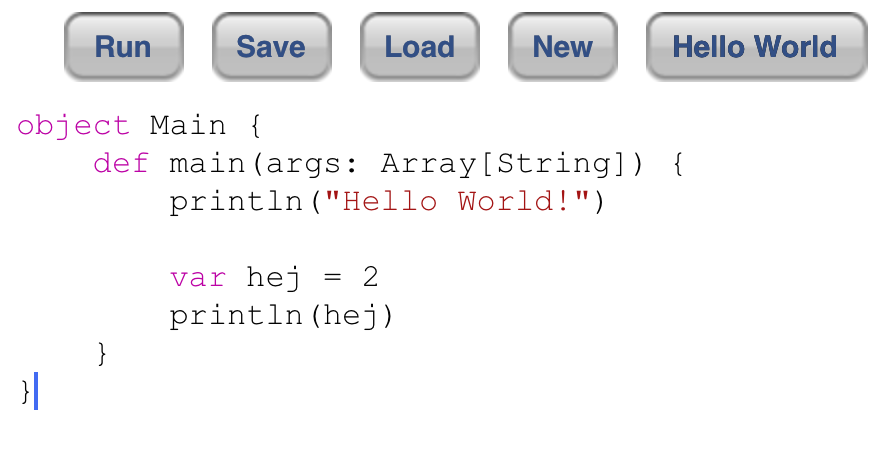
\includegraphics[width=80mm]{diagrams/CodeToGo_screenshot.PNG}
	\caption{The upper right corner of an example Scala program in CodeToGo.}
\label{fig:CodeToGo_screenshot}
\end{figure}

The most severe usability problem for CodeToGo is the low degree to which the user is able to recover from errors. If you have a syntax error in your code you will get a standard console compile error from the ideone.com server. This error contains the line number where your program failed, but when you dismiss the error you will have to remember this line number and manually count your way down to the line where the mistake was, as the editor does not display line numbers\,\cite{nielsen1990heuristic}.

The editor only has the aforementioned character selector as an accelerator for advanced users. Other than that there are no ways for users to improve when using the tool other than to learn to type faster on an iPad\,\cite{nielsen1990heuristic}.

Nielsen \todo{year} recommends that you follow the iOS platform standards so that the user does not have to put too much effort into learning how to use each app in a special way. Nielsen also recommends having undo support. CodeToGo does have undo support and follows the standard way of iOS, which is to shake the device. One could argue that shaking their iPad is not the most elegant way of allowing programmers to undo their typing, so in this case following the standards is not necessarily the best way to go for a mobile programming interface.

\paragraph{Takeaways}
\begin{enumerate}
	\item Do not assume that a virtual keyboard is as usable as a physical one\,\cite{nielsen2013mobile}. The touch interface has potential if you design your user experience to take advantage of it, but if you chose to ignore its potential/limitations you will have lower usability.
	\item You need accelerators for users to become faster and more comfortable with the interface. An accelerator could, for example, be auto completion and/or static checking.
	\item Undo support is essential for usability\,\cite{nielsen1990heuristic}, but if shaking the device is the right input method is questionable.
\end{enumerate}

\todo{Mention Dringend?}

\subsubsection{Textastic}
\label{subsub:Textastic}
Like CodeToGo, Textastic aims to be a general purpose programming editor, and as such supports many popular programming languages. Unlike CodeToGo, however, it does not support any way to run your code (besides manually copying your program to a computer and running the code there). Textastic is interesting due to an interface component that is not seen in CodeToGo.

\begin{figure}
	\centering
		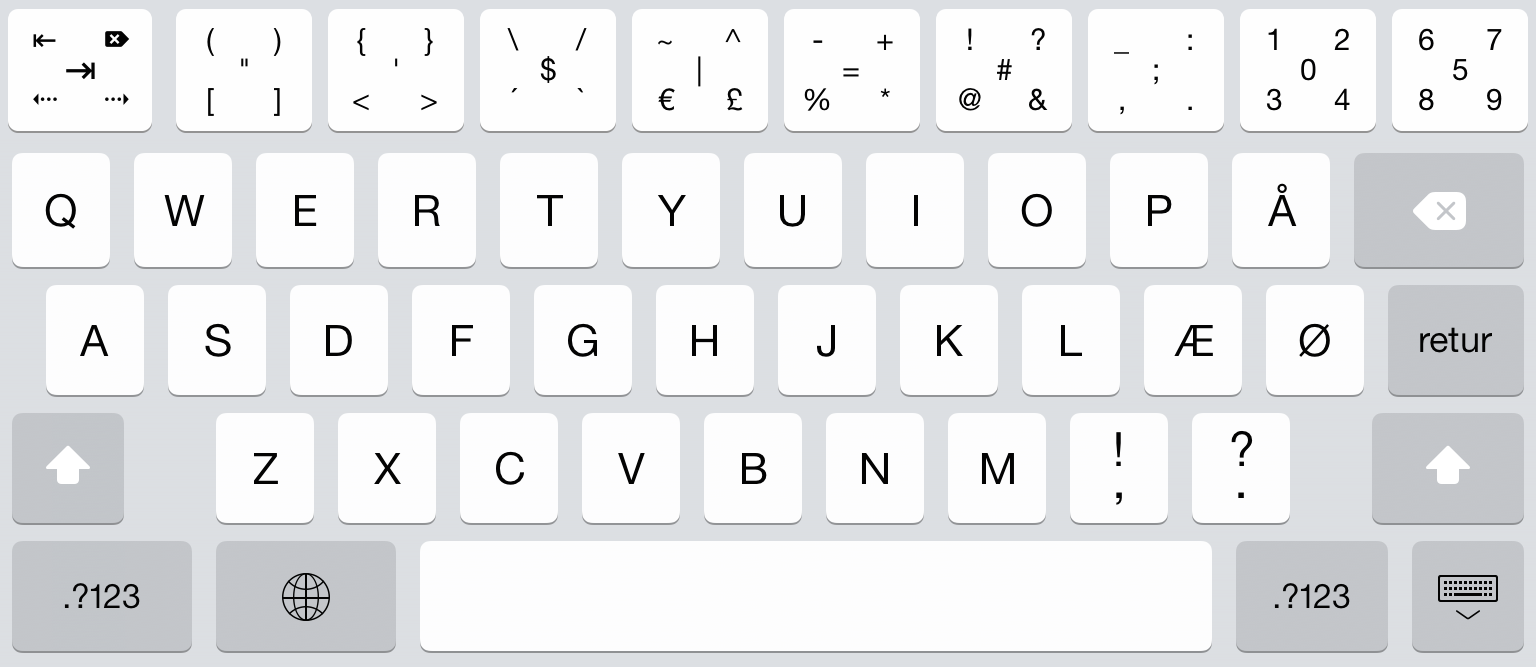
\includegraphics[width=110mm]{diagrams/textastic_keyboard_screenshot.png}
	\caption{The Textastic keyboard with special characters easily accessible.}
\label{fig:textastic_keyboard_screenshot}
\end{figure}

Textastic uses a smart shortcut bar that can be seen in Figure \ref{fig:textastic_keyboard_screenshot}. This bar allows quick access to commonly used characters, that would otherwise be hard to get to with the virtual keyboard. To select a special character you tap and hold your finger on the specific button and swipe towards the character that is needed. The biggest problem with Textastic is that you have no way of knowing whether your code will run or not.\todo{ref 10 heuristics. Specifically, user feedback} On a computer, this would not be as big of a problem, in fact many programming editors do not touch on the semantics of the language they are editing, instead they rely on other software to run the code. This is much harder on a device such as an iPad, where multitasking is not as prevalent. The text editing interface is very reminiscent of none-touch GUI text editors, such as TextMate or Sublime Text. 

\paragraph{Takeaways}
\begin{enumerate}
	\item Even in our IdrisTouch interface there will be a need for inputting special characters, and the solution Textastic has come up with is the most intuitive we have seen.
	\item It is not enough to have a good editing interface of your final product, if such a basic issue as running your code is unaddressed.
\end{enumerate}


\subsubsection{Raskell}
\label{subsub:Raskell}
Raskell is a Haskell editor for the iPad and a part of the UI can be see in Figure \ref{fig:Raskell_screenshot}. It is based on the Hugs implementation of Haskell 98, and includes the ability to interpret your programs locally. The text editor itself is inspired by Vi, featuring many of the same keyboard commands. When you have written your program, you can load it into the interpreter, which gives you a REPL, letting you test out your program. Raskell supports syntax highlighting for Haskell, and features most libraries for Hugs, but does not have auto completion.

The text editing itself works well, but a lack of auto completion and snippets mean you will be using the virtual keyboard to a large extent, which is generally a problem according to Nielsen\,\cite[pp. 76]{nielsen2013mobile}. 

\begin{figure}
	\centering
		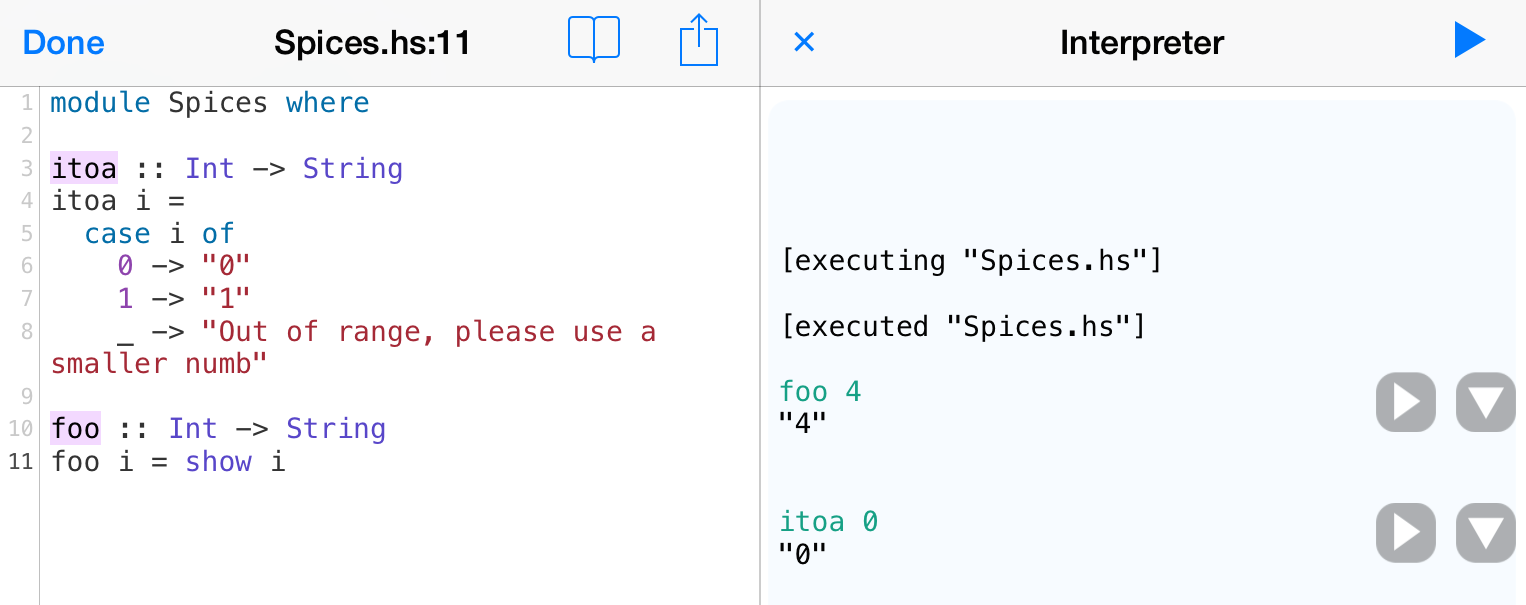
\includegraphics[width=110mm]{diagrams/Raskell_screenshot.png}
	\caption{The top of the Raskell environment with code editing to the right and a REPL to the
	left.}
\label{fig:Raskell_screenshot}
\end{figure}

Apart from this issue, the development flow is flexible and efficient. Especially compiler errors are being handled in an elegant way letting the user recover from syntactical errors\,\cite{nielsen1990heuristic}. If a compile error occurs, the user is presented with a split-screen view showing the error and a line number. The REPL is also extremely useful for trying out parts of your program.

Compared to CodeToGo, the Raskell development flow is quicker. This may be due to the local interpreter that evaluates your Haskell code as opposed to the network based approach CodeToGo takes. \todo{maybe insert something about the vim like keyboard?}

\paragraph{Takeaways}
\begin{enumerate}
	\item It is ideal to evaluate code locally as opposed to using a remote server.
	\item A solid way to recover from syntax errors is essential to a good development experience.
\end{enumerate}

\paragraph{}

For all of the three editors in this section there is one main problem: The heavy reliance on the virtual keyboard. Also, only using one type of touch-gesture (the single tap) seems like a wasted opportunity.
According to Nielsen it is important to optimize your solution for the touch
interface and not simply convert an existing desktop interface\,\cite[p 26, p
41]{nielsen2013mobile}.

One last issue that all of the above editors have in common is the lack of auto completion and user accelerators in general.

\subsection{Structured, Touch-Based Editors}
In this section we look at structured editor that, which are different from the previously mentioned editors in that the editors are cognizant of the underlying structure of the program, the abstract syntax tree (AST). The user more or less directly manipulates this AST, which is representing the given program.

\subsubsection{Lisping}
\label{subsub:Lisping}
Using the Scheme dialect of LISP you can program and execute code right on your iPad with Lisping. The idea is to take advantage of the close proximity between the abstract syntax tree and source syntax of LISP to edit code in a structured way. So you are actually manipulating the abstract syntax tree almost directly instead of having to type in every single character of every single line. While other iPad solutions run code on an external server, Lisping runs locally using a Scheme interpreter written in C, called TinyScheme. Lisping has been written with usability in mind\,\cite{lisping}: 

``Textviews and virtual keyboards aren't the only option for coding on iOS. Editing source code character by character is a concept wedded to the keyboard and it is not necessarily the best option for a device with no keyboard.''

Lisping is also a touch-based programming editor with support for multiple types of gestures, but it is the fact that it is structured that makes it interesting to our study.

We are fairly experienced programmers with only little knowledge of the Scheme language and it's syntax, and we had a hard time understanding and using Lisping. The underlying TinyScheme interpreter most often gave us “Error Unknown” compiler messages even though we were writing examples straight from the Scheme website. Not being able to pinpoint what was syntactically wrong with the written code and recover from that error was a major problem, as stated by Nielsen's ninth heuristic\,\cite{nielsen1990heuristic}.

The editor supports a range of touch gestures that are not immediately obvious to the user. Low memorability is generally a problem with touch gestures as described by Nielsen \cite[p. 141]{nielsen2013mobile}. In Lisping, you have to open the Lisping guide in the upper right corner and read through 6 pages of a PDF document to familiarize yourself with these gestures. This is a memorability problem\,\cite{nielsen1990heuristic}.

As can be seen in Figure \ref{fig:Lisping_screenshot}, there are also several buttons on the bottom of the UI. These are all icons and except for the delete and edit ones, they have no standard meaning in iOS or are used differently from the standard meaning. The undo button is e.g. a backwards-pointing triangle which could be interpreted to mean “Back” in iOS. Given the fact that the user has no chance of remembering all these non-standard icons, they clearly violate the ``Recognition rather than recall'' and ``Consistency and standards'' usability guidelines\,\cite{nielsen1990heuristic}. 

\begin{figure}
	\centering
		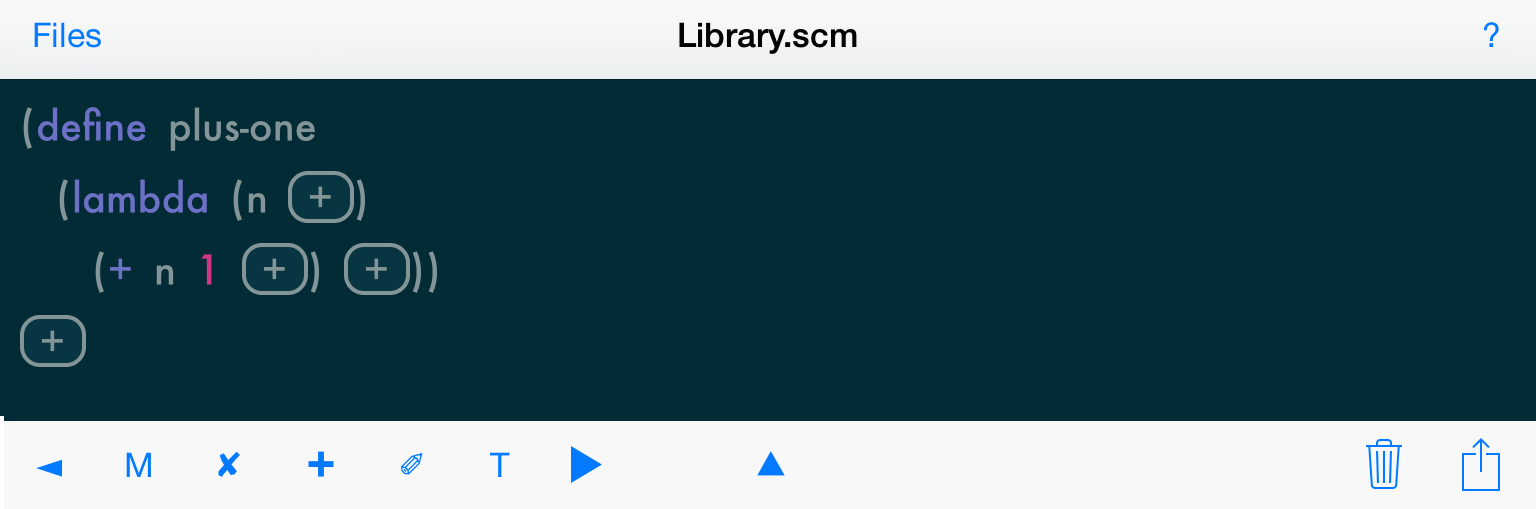
\includegraphics[width=110mm]{diagrams/Lisping_screenshot.png}
	\caption{A cropped screenshot of the Lisping interface, where the bottom
	toolbar consists of a range of non-standard icons and the program is filled
	with [+] buttons}
\label{fig:Lisping_screenshot}
\end{figure}

Furthermore, these icons are all located close to each other and a whole screen length away from where the user's attention is supposed to be when programming --- that is, on the code. All but two of the actions that these icons allow the user to do can be done with various gestures performed on the source code. We see this as a failed attempt on providing accelerators for the expert user.

The problem with these gestures is that they are uncomfortable and cumbersome to use. To select an expression to edit or run in the REPL, the user must ``reverse pinch'' the text. This is a non-standard way of highlighting text in iOS and it feels very awkward and unresponsive not to mention that it gets painful to do after three to four times. It is even straining to perform normal tap gestures due to the small size of all the expressions of the editor.

The final usability problem we discovered with Lisping was the amount of [+] buttons inlined in the code. These buttons are supposed to indicate that an expression can be added there, but what they also do is make the code much harder to read.
In Figure \ref{fig:Lisping_screenshot} we have a fairly simple program with
only three [+] buttons. This becomes more severe when the program grows.

\paragraph{Takeaways}
\begin{enumerate}
	\item The error messages from the compiler/interpreter should indicate where in the code the syntax errors have occurred. Simply presenting “Unknown Error” is frustrating for the user.
	\item It should not be necessary to add a PDF documents with instructions to how the gestures and buttons work. It should be immediately recognized by the user because it is all presented according to the platform standards. This serves as a reminder that the overuse of clever gestures harms the user experience.
	\item Littering a structured editor with [+] (add) buttons, to indicate that expressions can be added at these positions, is not a good idea. While a good alternative for this solution is hard to come up with we should try to design a different way.
\end{enumerate}

\subsubsection{Eastwest}
\label{subsub:Eastwest}
Even though Eastwest is basically an experiment, we find it very interesting. It is a structured editor for a functional language that allows the user to ``fill in holes'' i.e. fulfill goals of a program from a context. The context appears right under the goal and thus works as a well-placed auto completion tool. We have been unable to complete a heuristics evaluation of Eastwest, as we were unable to install it on our computers. Several videos are available, though, and it is interesting to see how functional data types are being defined and functions are being built in a structured way. \todo{insert reference}
\todo{Eastwest is not touch-based?}

\paragraph{Takeaways}
\begin{enumerate}
	\item Having a context close to the goal makes for quick and easy access. The better that context is at guessing the right thing for the goal, the faster the tool will seem.
	\item EastWest is a good indication that functional languages work well in a structured editor.\todo{do we mean strongly/statically typed languages?}
\end{enumerate}


\subsubsection{TouchDevelop}
\label{subsub:TouchDevelop}
TouchDevelop allows developers to make touch and accelerometer enabled games for any device with a web browser by providing a web app. It is generally meant as a way of getting youngsters interested in programming, and the language has been specially designed for this purpose and works hand in hand with the development platform to provide a good experience for touch devices.\todo{insert ref for touchdev}

TouchDevelop is not general purpose but focuses on creating simple 2D games. This means that the user gets a lot of standard game concepts built into whatever program he's writing. This is evident from the context that is being updated as you type in the bottom of the screen. This basically means that you rarely have to type characters into the editor as you don't have to define new methods (actions). Variable names are automatically generated at the push of a button.
Figure \ref{fig:TouchDevelop_screenshot} shows a sample program drawing a
turtle and a simple triangle pattern.

\begin{figure}
	\centering
		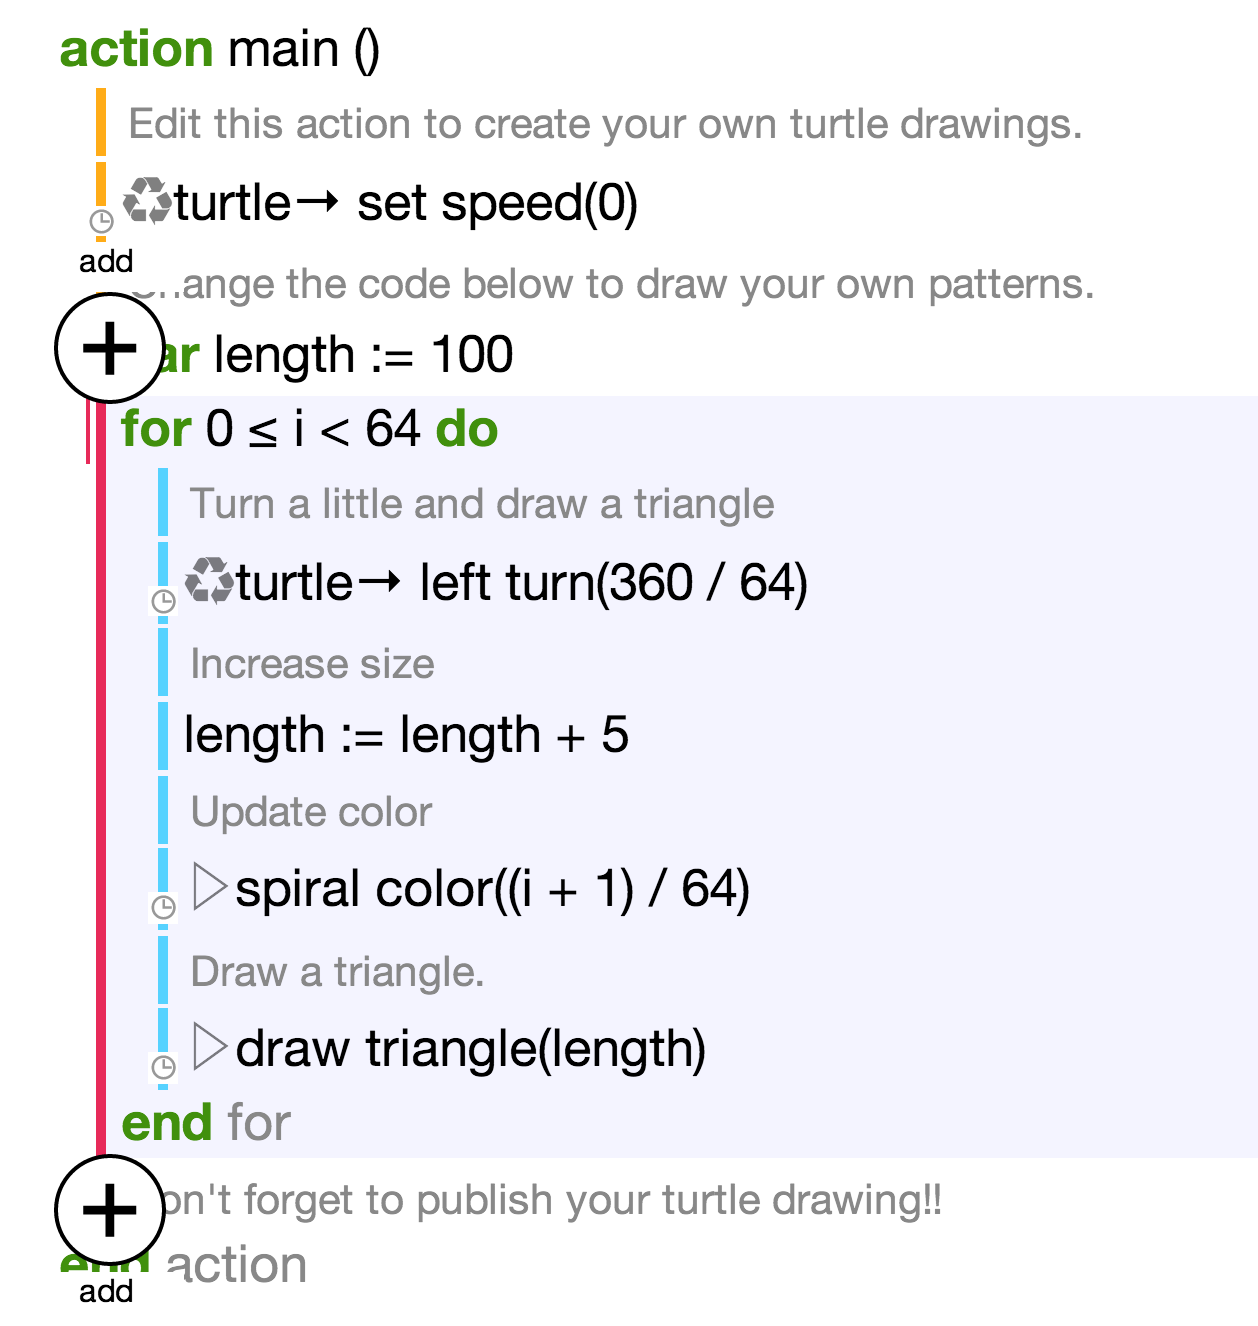
\includegraphics[width=80mm]{diagrams/TouchDevelop_screenshot.png}
	\caption{A screenshot of the Turtle Triangle Spiral sample from
	TouchDevelop\,\cite{TouchDevelop:TurtleTriangleSpiral}}
\label{fig:TouchDevelop_screenshot}
\end{figure}

The first thing you notice as an experienced programmer is how the TouchDevelop language looks like modern imperative languages like C\# and Java, and this recognizability enabled us to get started with the platform right away. To educate new users there is a long tutorial that guides you through your first game. This tutorial makes the language seem very structured but in fact it is as easy to make syntactical error as in any other imperative language. We have placed TouchDevelop in this section of structured editors even though it should only be categorized as semi-structured.
\todo{should it?}

Even though TouchDevelop works on all touch devices that has a web browser it is not really optimized for other gestures than the standard single tap gesture that works on all platforms.

To fit more code on the screen and create a better programming overview, TouchDevelop uses a rather small font for the code you write. When you tap the line of code you wish to edit, that statement is enlarged and you can relatively easily move the cursor around. Additionally, buttons appear to insert new lines above and below the selected segment. This design is minimalistic and controls only show up when you need them\,\cite{nielsen1990heuristic}.

The context that is presented to the user to select method calls and objects from is convenient when it presents you with just what you needed, but in most cases you find yourself struggling to find just that. This is due to the nature of object oriented languages. When filling out a hole in the program, the type system cannot narrow down the possibilities, as any object could potentially allow the user to create the right type according to the compiler. This seems to be a problem for us as novice users given the vast number of elements in the context at any given time slows down our programming speed.

The feel of TouchDevelop suffers from the fact that it is a web app written with no specific platform in mind. The biggest annoyance is when you want to move around the cursor. This is clumsy on the iPad and often requires that you use buttons.

\paragraph{Takeaways}
\begin{enumerate}
	\item To have a contextual overview can speed up the tasks of programming just as we saw with Eastwest.
	\item The type system of the TouchDevelop object oriented programming language is not ideal if you want to expose a context for the user to pick from. The type system simply can't narrow down the possibilities efficiently.
	\item Using a smaller font for code that is not in focus is a clever way to create a better overview for the user.
	\item There is a clear difference between the feel of a web app like TouchDevelop and a native app like Lisping.
\end{enumerate}

\paragraph{}

The more structured the touch-based editor is, the more well-functioning auto completion seems to be on touch devices. As we have learned, it is paramount to have as little use of the virtual keyboard as possible and adopting the structured approach together with the strong type system of Idris should be able to give us just that.

\subsection{Existing Solutions Overview}
Table \ref{table:existing_solutions_overview} gives an overview of the existing solutions and how we will be positioning our IdrisTouch solution compared to these. Our study indicates that touch gestures can be used as accelerators for super users, so we will have focus on implementing these where it makes sense. The strong type system of Idris allows us to make a more structured editor than most existing solutions. Lastly, it is our theory that we can represent Idris data types in a more visual way than what programmers are used to from the current concrete syntax.
	
% Please add the following required packages to your document preamble:
% \usepackage{multirow}
% \usepackage[table,xcdraw]{xcolor}
% If you use beamer only pass "xcolor=table" option, i.e. \documentclass[xcolor=table]{beamer}

\begin{table}[ht]
{\renewcommand{\arraystretch}{2}%
\begin{tabularx}{\textwidth{}}{|c|X|c|c|c|}
\hline
	& \textbf{Description}
	& \textbf{Touch-based}                                              
	& \textbf{Visual syntax}                          
	& \textbf{Stuctured editor} 
\\ \hline		
	\textbf{Labview}      & 
		Visual data flow programming & & \cellcolor[HTML]{38761D} &
\\ \hline
	\textbf{Scratch}      & 
		Beginner-friendly programming by dragging boxes
		  & & \cellcolor[HTML]{274E13} & \cellcolor[HTML]{274E13}
\\ \hline
	\textbf{Epigram}      & 
		Functional with Dependent Types & & \cellcolor[HTML]{6AA84F} &
\\ \hline
	\textbf{CodeToGo} & & \cellcolor[HTML]{B6D7A8}{\color[HTML]{9AFF99} }                  & & \\ \cline{1-1}
	\textbf{Textastic}  & \multirow{-2}{*}{
	Textual iPad env.
	} & \multirow{-2}{*}{\cellcolor[HTML]{B6D7A8}{\color[HTML]{9AFF99} }} & \multirow{-2}{*}{}                              & \multirow{-2}{*}{}                                                   
\\ \hline
	\textbf{Raskell}      & 
		Mobile Haskell & \cellcolor[HTML]{B6D7A8}{\color[HTML]{9AFF99} } & &                                                               
\\ \hline
	\textbf{Lisping}      & 
		Mobile Lisp & \cellcolor[HTML]{6AA84F} & & \cellcolor[HTML]{B6D7A8}

\\ \hline
	\textbf{Eastwest}     & 
		Functional programming system with structured editor
		 & & & \cellcolor[HTML]{274E13}
\\ \hline	
	\textbf{TouchDevelop} & 
		Imperative language running as a web app
		 & \cellcolor[HTML]{6AA84F} & & \cellcolor[HTML]{B6D7A8} 
\\ \hline
	\textbf{IdrisTouch}   & 
		Mobile Idris      & \cellcolor[HTML]{38761D} & \cellcolor[HTML]{6AA84F}           & \cellcolor[HTML]{38761D} 
\\ \hline
\end{tabularx}
}
\caption{Existing solutions overview.}
\label{table:existing_solutions_overview}
\end{table}

\subsection{Overall Takeaways}
In this section we have analyzed a range of existing solutions and for each reached a list of takeaways that we'll be using to form our requirements for the IdrisTouch app.

We learned that visual elements can help structure a programming language and its environment, but that the most successful VPLs so far have been domain specific. Idris is a general purpose language so it will be a challenge to incorporate simple visual elements to enhance the user experience.

The current state of the art touch-based iPad apps either only use the single tap gesture, thus wasting a golden opportunity, or use several gestures without concern for the usability of them. The issue seems to be that they are all essentially manipulating text and that the standard text input UI elements on the iPad already support several gestures. If the app tries to incorporate too many gestures to manipulate the structure of these text fields there may be conflicts. Finding a solution to this problem is another major challenge.

Finally, we discussed a few structured editors where two of them support functional languages. Having the editor be cognizant of the underlying structure of the program seems to lessen the amount of typing the user has to perform on the virtual keyboard. Furthermore, the stronger the type system is and the purer the underlying language, the less the programmer has to type, as type inference becomes better. The IdrisTouch editor should be structured for these reasons.
